%!TEX root = ../thesis.tex
%*******************************************************************************
%****************************** Fourth Chapter *********************************
%*******************************************************************************

\ifpdf
    \graphicspath{{Chapter4/Figs/PDF/}{Chapter4/Figs/Raster/}{Chapter4/Figs/}}
\else
    \graphicspath{{Chapter4/Figs/Vector/}{Chapter4/Figs/}}
\fi

\chapter{Current work}
\label{ch:diagnostic_results_discussion}
\label{ch:diagnostic_results}

Chapter~3 defined the controlled SENT benchmark, the phase-field fatigue formulation, the FEM reference, the PIDL formulation and the FEM–PIDL alignment protocol. This chapter reports the diagnostic results from that benchmark. The purpose is not to validate pavement-level road-crack prediction. The study is still a controlled numerical fracture benchmark with known geometry, loading, material parameters and initial crack state. Rather than only reporting the numerical mismatch, it explains the diagnostic process used to make the mismatch interpretable.



\section{Purpose and Diagnostic Definitions}
\label{sec:c4_diagnostic_definitions}

The state-variable storage and update conventions used in the following diagnostics were defined in Chapter~3. In particular, Table~\ref{tab:c3_state_variable_storage_update_audit} states where the main FEM and PIDL quantities are stored, how Gauss-point FEM quantities are reduced for comparison with PIDL elementwise diagnostics, and when the active driver, fatigue history and fatigue degradation are updated. Chapter~4 therefore does not redefine the update algorithm. It uses that audit table as the reproducibility basis for the field-level comparisons below.

The comparison is FEM-first. A ratio greater than one therefore means PIDL overprediction relative to FEM, while a ratio below one means PIDL underprediction relative to FEM. Field comparisons use committed diagnostic states, not intermediate trial states during optimisation or staggered solution.

\begin{table}[!htb]
\centering
\caption{Diagnostic definitions used in the FEM--PIDL fatigue comparison.}
\label{tab:c4_diagnostic_definitions}
\begin{tabular}{p{0.24\textwidth} p{0.52\textwidth} p{0.16\textwidth}}
\hline
\textbf{Diagnostic quantity} & \textbf{Definition used in this chapter} & \textbf{Level} \\
\hline
Fatigue life, \(N_f\)
& First committed cycle at which the prescribed crack-event criterion is satisfied.
& Scalar \\

Crack-event criterion
& Fixed damage-threshold and connectivity rule used to identify whether the crack has reached the selected event condition. The same rule is applied to FEM and PIDL fields after the stated spatial mapping.
& Damage field \\

Event cycle
& First cycle satisfying the crack-event criterion. FEM and PIDL event cycles are reported separately; mapped-state comparisons also use the FEM event cycle as a reference state.
& Scalar / state label \\

Crack-tip position
& Most advanced point of the connected damaged region under the same threshold and connectivity rule.
& Spatial \\

Crack-tip error
& Distance between FEM and PIDL crack-tip positions at the same committed state or at the mapped event state.
& Spatial \\

Process-zone region
& Local region around the crack tip or high-driver zone used for field statistics. The same mask or distance rule is used before field ratios are interpreted.
& Elem / field \\

Field ratio
& PIDL value divided by FEM value for the same diagnostic field, same state label and same spatial reduction.
& Scalar statistic \\

High-percentile field statistic
& Percentile reduction, usually \(99\)th percentile, used to compare field distributions without relying only on maxima.
& Field statistic \\

Energy ratio
& PIDL/FEM ratio for the same energy contribution, usually \(E_{\mathrm{el}}\) or \(E_{\mathrm{d}}\), at a stated cycle or mapped event state.
& Scalar \\
\hline
\end{tabular}
\end{table}



\section{Scalar Fatigue-life Agreement Versus Local Field Mismatch}
\label{sec:c4_early_scalar_feasibility}

The first result was a scalar fatigue-life sweep. It tested whether the PIDL formulation could reproduce the broad relationship between displacement amplitude and cycles to the event criterion. Figure~\ref{fig:c4_pre_alignment_nf_sweep} shows that the PIDL runs followed the same monotone $U_{\max}$–$N_f$ trend as the FEM reference, while the gap is larger at lower displacement amplitudes. This result showed that the PIDL fatigue formulation was able to capture part of the global fatigue-life response.

\begin{figure}[!htbp]
    \centering
    \includegraphics[width=0.78\textwidth]{c4_pre_alignment_nf_sweep.pdf}
    \caption{Exploratory \(U_{\max}\)--\(N_f\) sweep. The PIDL run follows the same monotone fatigue-life trend as the FEM reference, while the gap is larger at lower displacement amplitudes.}
    \label{fig:c4_pre_alignment_nf_sweep}
\end{figure}

% \begin{table}[!htbp]
% \centering
% \caption{Exploratory scalar sweep.}
% \label{tab:c4_pre_alignment_nf_sweep}
% {\small
% \begin{tabular}{cccc}
% \hline
% \(U_{\max}\) & FEM \(N_f\) & PIDL \(N_f\) & PIDL/FEM \\
% \hline
% 0.08 & 396 & 341 & 0.86 \\
% 0.09 & 254 & 230 & 0.91 \\
% 0.10 & 170 & 160 & 0.94 \\
% 0.11 & 117 & 112 & 0.96 \\
% 0.12 & 82  & 80  & 0.98 \\
% \hline
% \end{tabular}
% }
% \end{table}

However, the interpretation changed when local fatigue fields were examined. Figure~\ref{fig:c4_pre_alignment_dispersed_degradation} shows that the early PIDL runs could appear close to the FEM reference at the scalar \(N_f\) level, while following a different degradation path. The FEM reference showed stronger late local degradation, whereas the PIDL curves degraded more gradually over the normalised cycle range. This implies that the PIDL model was not concentrating fatigue degradation in the same crack-tip process zone as the FEM calculation. This observation is supported by the single-amplitude diagnostic in Figure~\ref{fig:c4_pre_alignment_u012_internal_diagnostics}. At $U_{\max}=0.12$, the exploratory fracture-cycle estimates were close, with FEM $N_f=82$ and the three PIDL seeds giving $N_f=81$, $86$ and $81$. However, the internal fatigue-history and degradation fields were not matched. This is the key diagnostic trigger for the rest of the chapter: similar scalar event timing can be obtained even when the hidden fracture-state fields are not FEM-like.

\begin{figure}[!htb]
    \centering
    \includegraphics[width=0.95\textwidth]{c4_pre_alignment_dispersed_degradation.pdf}
    \caption{Early comparison of minimum fatigue-degradation evolution. The figure is used as diagnostic evidence only: it explains why scalar \(N_f\) agreement was not sufficient and why local neural-network representation was investigated in the diagnostic workflow.}
    \label{fig:c4_pre_alignment_dispersed_degradation}
\end{figure}



% Instead, it yields highly dispersed local fields that under-resolve the steep gradients required to correctly simulate crack propagation.


% The FEM peak \(\bar{\alpha}_{\max}\) is approximately \(958\), while the PIDL values are approximately \(9\)--\(14\) and more spatially dispersed. 


\begin{figure}[!htb]
    \centering    \includegraphics[width=0.9\textwidth]{c4_pre_alignment_u012_internal_diagnostics.pdf}
    \caption{Early single-amplitude diagnostic at \(U_{\max}=0.12\). The fracture-cycle estimates are close in this exploratory plot (FEM \(N_f=82\); PIDL seeds \(N_f=81,86,81\)), but the internal fatigue-history and degradation quantities are not matched. This figure should be treated as exploratory evidence rather than final mechanism evidence.}
    \label{fig:c4_pre_alignment_u012_internal_diagnostics}
\end{figure}


The scalar sweep is therefore treated as a starting point rather than a validation result. It showed that the PIDL formulation was not unrelated to the FEM fatigue response, but it did not show that the same fatigue mechanism was being reproduced. The rest of the chapter therefore moves from scalar event timing to energy, fatigue-history, degradation, active-driver and process-zone diagnostics.


% \section{Field-level Mechanism Diagnosis}
% \label{sec:c4_fatigue_benchmark}

% This section gives the retained field-level diagnosis from the aligned cyclic benchmark. The comparison uses the protocol defined in Chapter~3 and the diagnostic definitions in Table \ref{tab:c4_diagnostic_definitions}. The aim is to identify which part of the fatigue-fracture chain fails. The evidence is organised from global response to local mechanism: first the late-cycle energy divergence, then fatigue-history and degradation fields, then raw and active crack-driving fields, and finally process-zone and crack-tip lag.

% \subsection{Late-cycle Global Response Divergence}
% \label{sec:c4_late_cycle_global_divergence}

% The late-cycle global response is the first central failure mode. The early energy response is close: at the first peak loading state, the PIDL-to-FEM elastic-energy ratio is approximately \(0.991\), and the corresponding damage-energy ratio is approximately \(0.955\). These values support the interpretation that the two calculations begin with a comparable energy scale under the aligned benchmark. 

% By the FEM crack-event cycle, the response has diverged strongly. In the retained active-driver PIDL run, the corresponding event is delayed, with the first and confirmed event detections occurring later than the FEM event cycle. At the FEM event-cycle comparison state, the PIDL-to-FEM elastic-energy ratio increases to approximately $4.789$, while the damage-energy ratio falls to approximately $0.448$. The PIDL solution therefore stores too much elastic energy and develops too little damage energy at the late fracture stage.



% The previous section showed that changing the PIDL architecture or adding local features could alter event timing and local field patterns, but failed to reliably remove the field mismatch. This implies that the bottleneck is not simply a matter of network capacity, but is probably rooted in how the fields change over time. Therefore, this section tried to track the continuous evolution trajectories of the field variables. We investigate whether the coupled fracture and fatigue fields in the PIDL framework evolve in the same way as the FEM reference and make the field disagreements physically interpretable.

% During this exploration, we found that the fatigue comparison required extra care because cyclic fracture evolution depends heavily on state history. Small differences in boundary conditions or initial states can change the stress-localisation patterns near the pre-crack, altering where fatigue history accumulates during loading. So the initial state was checked  first.


% \subsection{Initial-State Verification}
% \label{sec:c4_initial_state}

% The comparison uses two solvers of the same controlled SENT specimen under repeated loading with a displacement amplitude of 0.12. The FEM simulation provides the controlled phase-field fracture reference. The PIDL model is trained and evaluated on the corresponding setting. 


% % This section took a sticker alignment on the crack state, boundary conditions, material and fatigue laws, mesh mapping and loading-state convention. These checks are summarised in Table~\ref{tab:c4_alignment_checks}. 

% % \begin{table}[!htb]
% % \centering
% % \caption{Alignment checks used for the FEM--PIDL fatigue benchmark.}
% % \label{tab:c4_alignment_checks}
% % {\small
% % \setlength{\tabcolsep}{5pt}
% % \begin{tabular}{p{0.24\textwidth}p{0.66\textwidth}}
% % \hline
% % Check & Evidence and role in the comparison \\
% % \hline
% % Crack state & Both models use the same diffuse representation of the initial horizontal pre-crack, reducing ambiguity from inconsistent crack initialisation. \\
% % Boundary conditions & Support and loading compatibility were checked to reduce stress-localisation confounds in the vertical displacement-controlled SENT setup. \\
% % Material/fatigue laws & The material parameters and fatigue-degradation law defined in Chapter~3 are used; initially \(\bar{\alpha}=0\) and \(f_{\mathrm{fatigue}}=1\). \\
% % Mesh/probe mapping & PIDL triangles are area-averaged onto FEM elements before residuals and scalar reductions, so fields are compared on a common spatial support. \\
% % State matching & Labelled peak and unloaded states are compared, avoiding raw output-index comparisons within the loading cycle. \\
% % Monotonic sanity check & The basic phase-field setup was checked before cyclic fatigue interpretation; this check is treated as alignment evidence, not as fatigue validation. \\
% % \hline
% % \end{tabular}
% % }
% % \end{table}

% % \textcolor{red}{
% % Spatial mapping was also considered here. FEM fields were exported on quadrilateral element means, while PIDL fields were evaluated on triangular elements. PIDL coordinates were shifted into the FEM frame and area-averaged onto the FEM element grid before residuals were computed. Loading states were compared by physical state labels, such as peak and unloaded states, rather than by raw output indices. This avoids artificial comparisons between different positions within the loading cycle.}



% % \begin{figure}[!htb]
% %     \centering
% %     \includegraphics[width=\textwidth]{c4_sent_probe_zone_schematic.pdf}
% %     \caption{Schematic of the controlled SENT benchmark and the comparison regions used in the diagnostic reductions. The figure is not to scale. It indicates the cyclic displacement setting, the initial horizontal pre-crack, the common probe line, the crack-tip region and the right-side event region used to interpret field and scalar evidence.}
% %     \label{fig:c4_sent_probe_zone_schematic}
% % \end{figure}


% It is noted that the initial-crack treatment was revised to make the FEM and PIDL settings more directly comparable. In the previous FEM setup, the pre-crack region was initialised as a fully damaged band while the fatigue history was set to zero, and the model was then relaxed under zero displacement before cyclic loading. Here, the FEM reference uses the same smooth diffuse initial-crack profile as the PIDL setting, with zero initial fatigue history, and then proceeds directly to the prescribed cyclic loading sequence.

% The initial-state comparison confirms that the starting fields are effectively matched. The maximum damage values in FEM and PIDL are both approximately \(0.905\), and the mean damage values are both approximately \(0.0378\). The fatigue-history variable is zero in both models, and the fatigue-degradation function \(f_{\mathrm{fatigue}}\) is initially equal to one.

% \textcolor{red}{need a residual figure for initial state here}

% This initial agreement does not guarantee field-level agreement during fatigue loading. It only shows that the later divergence is not caused by an obvious mismatch in the initial damage field, fatigue-history field or degradation state. The later comparison can therefore be interpreted as a fatigue-evolution problem rather than as an initial-state artefact.



% % \begin{table}[!htb]
% % \centering
% % \caption{Summary of the final aligned FEM--PIDL diagnostic comparison.}
% % \label{tab:c4_retained_benchmark}
% % \begin{tabular}{p{0.25\textwidth}p{0.65\textwidth}}
% % \hline
% % Item & Role in the diagnostic comparison \\
% % \hline
% % FEM reference & Provides the controlled phase-field fracture response under repeated loading. \\
% % PIDL run & Tests whether the fatigue-augmented PIDL formulation can reproduce the corresponding fracture-state evolution. \\
% % Initial crack state & Same diffuse representation of the initial horizontal pre-crack in FEM and PIDL. \\
% % Loading & Cyclic displacement-controlled tension with \(U_{\max}=0.12\) and minimum-to-maximum displacement ratio \(R=0\). \\
% % State comparison & Fields compared at corresponding loading states within the repeated-loading sequence. \\
% % Spatial comparison & PIDL fields mapped onto the FEM element grid before scalar reductions and residual fields are computed. \\
% % Main diagnostic target & Agreement in both scalar indicators and local fracture-state fields. \\
% % \hline
% % \end{tabular}
% % \end{table}

% \subsection{Global Scalar Divergence and Event-Timing Lag}
% \label{sec:c4_scalar_divergence_event_lag}

% The scalar comparison was examined in the initial-state verification. These scalar quantities test whether the PIDL run follows the broad fatigue progression of the FEM reference before the local fields are interpreted.

% The FEM reference reaches the crack-event criterion at cycle 69. The PIDL run detects the corresponding event later than the FEM reference. This timing difference is not so large that the PIDL response is unrelated to the FEM response, but it shows that the cyclic propagation process is delayed in the PIDL formulation.

% The early energy response is close. At the first peak loading state, the PIDL-to-FEM elastic-energy ratio is approximately \(0.991\), and the corresponding crack-surface-energy ratio is approximately \(0.955\). These values support the interpretation that the early loading response and energy scale are not obviously inconsistent.

% The late-cycle energy response is different. By the FEM crack-event cycle, the PIDL-to-FEM elastic-energy ratio increases to approximately \(4.789\), while the crack-surface-energy ratio falls to approximately \(0.448\). The PIDL run therefore carries too much elastic energy and accumulates too little crack-surface energy relative to the FEM reference near the late fracture stage.

% \begin{table}[!htb]
% \centering
% \caption{Selected scalar indicators from the FEM--PIDL fatigue comparison.}
% \label{tab:c4_scalar_indicators}
% {\small
% \begin{tabular}{p{0.24\textwidth}p{0.31\textwidth}p{0.34\textwidth}}
% \hline
% Quantity & Early-cycle comparison & Late-cycle comparison \\
% \hline
% Damage maximum & FEM/PIDL both approximately \(0.905\) initially & Similar order, but not sufficient to indicate field agreement \\
% Damage mean & FEM/PIDL both approximately \(0.0378\) initially & Comparable global mean, but local differences remain \\
% Elastic energy & PIDL/FEM ratio \(0.991\) at first peak & PIDL/FEM ratio \(4.789\) at the FEM event cycle \\
% Crack-surface energy & PIDL/FEM ratio \(0.955\) at first peak & PIDL/FEM ratio \(0.448\) at the FEM event cycle \\
% Event timing & Not applicable at initial state & FEM reaches event at cycle 69; PIDL event occurs later \\
% \hline
% \end{tabular}
% }
% \end{table}

% \begin{table}[!htbp]
% \centering
% \caption{Result-facing audit of fatigue-history and driver quantities used in Chapter~4.}
% \label{tab:c4_update_audit_summary}
% \begin{tabular}{p{0.18\textwidth} p{0.27\textwidth} p{0.27\textwidth} p{0.20\textwidth}}
% \hline
% \textbf{Quantity} & \textbf{FEM treatment} & \textbf{PIDL treatment} & \textbf{Diagnostic implication} \\
% \hline
% Damage \(\alpha\)
% & Nodal phase-field damage \texttt{p\_field}; interpolated to GP during assembly and reduced for field comparison.
% & Neural damage output \texttt{alpha}; evaluated at nodes and reduced to \texttt{alpha\_elem} for element diagnostics.
% & Defines the current crack state and process-zone map. \\

% Damage history
% & Committed nodal maximum damage \texttt{p\_field\_old}.
% & Committed nodal maximum damage \texttt{hist\_alpha}.
% & Correct pair for irreversibility-state comparison. FEM \texttt{history\_vars(:,:,1)} is not used as PIDL damage history. \\

% Raw driver \(\psi_{\mathrm{raw}}\)
% & Undegraded tensile driver \texttt{strain\_en\_undgr}; GP quantity reduced to element level.
% & \texttt{psi\_raw\_elem}; elementwise diagnostic.
% & Similar raw-driver maxima do not prove fatigue-mechanism agreement. \\

% Active driver \(\psi_{\mathrm{active}}\)
% & \(g(d_q)Y_q\) at GP level, reduced for comparison.
% & \texttt{psi\_active\_elem} or probe-reduced element diagnostic.
% & Central quantity for fatigue-history accumulation. \\

% Accumulated fatigue history \(\bar{\alpha}\)
% & \texttt{history\_vars(:,:,2)}; GP quantity reduced to element level.
% & \texttt{hist\_fat} or \texttt{alpha\_bar}; elementwise history.
% & Main underpredicted field in the PIDL result. \\

% Fatigue degradation \(f_{\mathrm{fatigue}}\)
% & \texttt{history\_vars(:,:,4)}; GP quantity reduced to element level.
% & \texttt{f\_fatigue}; elementwise degradation factor.
% & Controls effective damage-energy resistance. \\

% Current fatigue increment
% & Positive increment from the current active driver relative to previous GP baseline.
% & Use \texttt{delta\_alpha\_bar\_input\_elem}; saved \texttt{psi\_plus\_prev\_elem} may already be the next-step baseline.
% & Avoids misreading the saved baseline as the current increment. \\
% \hline
% \end{tabular}
% \end{table}

% \subsection{Field-Level Mechanism Diagnostics}
% \label{sec:c4_mechanism_diagnostics}

% The field-level comparison shows that the scalar divergence is associated with fatigue-history and degradation mismatch near the process zone. At the FEM event cycle, the maximum fatigue-history value in the FEM reference is approximately \(19.53\), while the corresponding PIDL value is approximately \(2.00\). The minimum fatigue-degradation value is approximately \(0.0146\) in FEM and  \(0.170\) in PIDL. Since smaller values of \(f_{\mathrm{fatigue}}\) indicate stronger local fatigue weakening, the PIDL formulation does not accumulate or degrade the local fatigue state as strongly as the FEM reference.

% The excessive late-cycle elastic energy is consistent with an under-developed local damage process zone in the PIDL solution. In the FEM reference, fatigue-history accumulation near the crack tip reduces \(f_{\mathrm{fatigue}}\), lowers the effective damage-energy resistance and allows stronger local damage growth. This reduces the local stiffness and increases the damage-energy contribution associated with crack-surface formation. In the PIDL result, fatigue-history accumulation and fatigue degradation remain weaker near the corresponding process zone. Under the same imposed displacement, the PIDL solution therefore retains a larger part of the response in the elastic-energy term and develops a smaller damage-energy contribution. This interpretation is supported by the late-cycle ratios \(E_{\mathrm{el}}^{\mathrm{PIDL}}/E_{\mathrm{el}}^{\mathrm{FEM}}\approx 4.789\) and \(E_{\mathrm{d}}^{\mathrm{PIDL}}/E_{\mathrm{d}}^{\mathrm{FEM}}\approx 0.448\), together with the underprediction of \(\bar{\alpha}\) and weaker fatigue degradation.

% \begin{figure}[!htb]
%     \centering
%     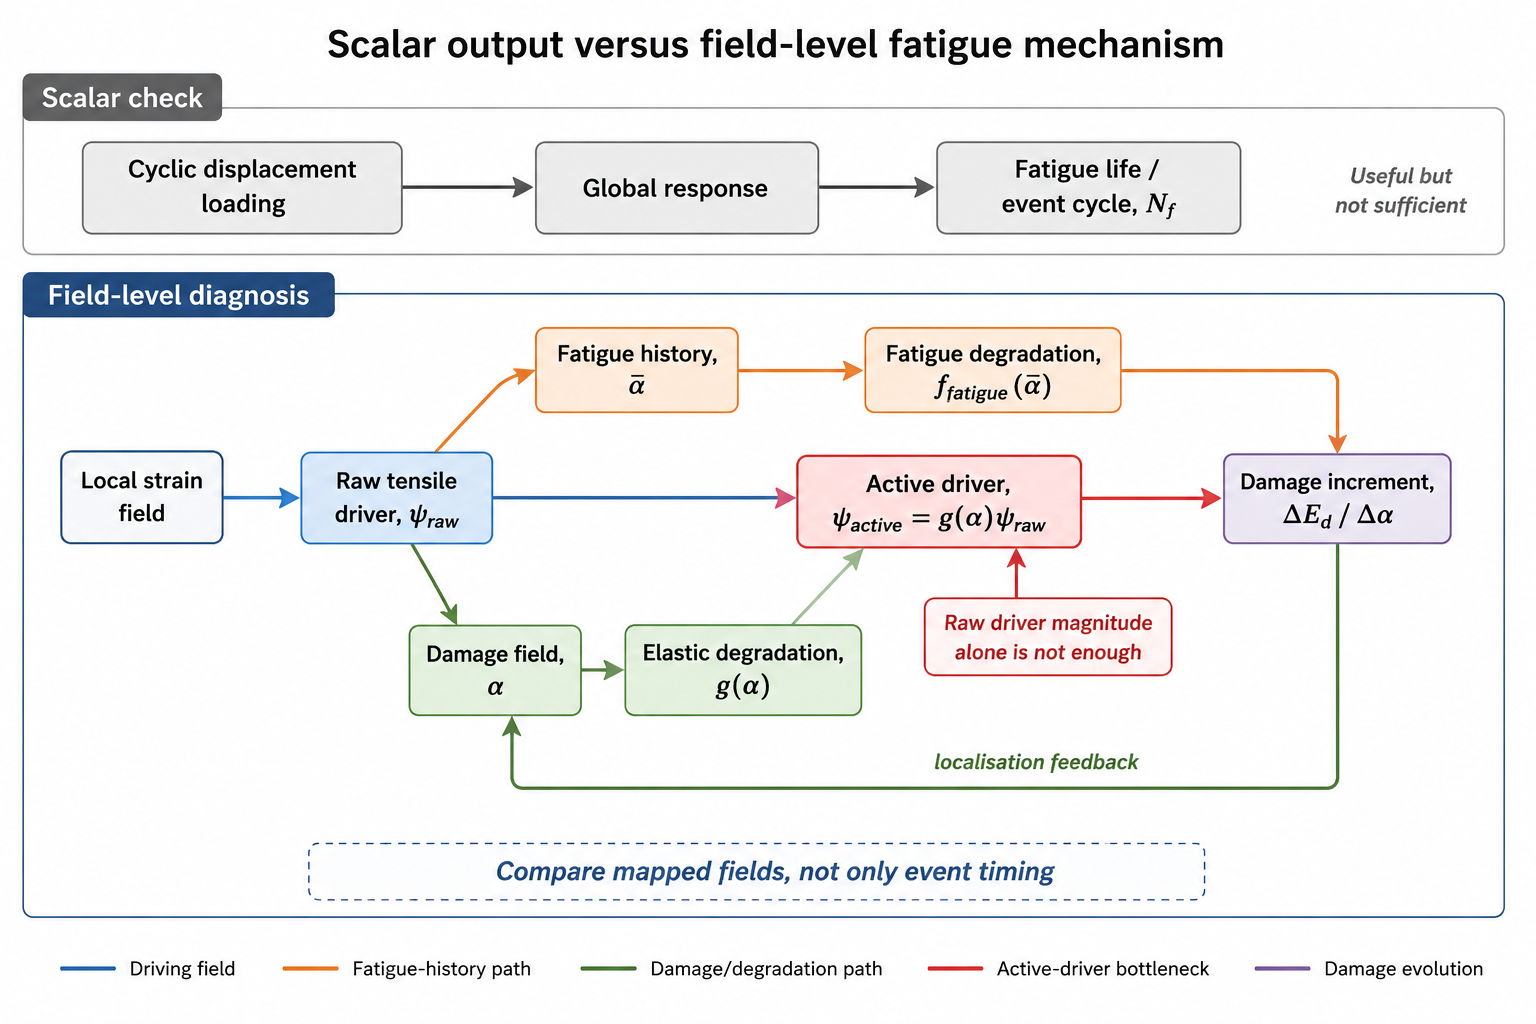
\includegraphics[width=\textwidth]{Chapter4/Figs/PDF/c4_phase_field_variable_map.png}
%     \caption{Coupled phase-field fatigue variables used in the FEM--PIDL comparison. The raw tensile driver \(\psi_{\mathrm{raw}}\), damage field \(\alpha\), fatigue history \(\bar{\alpha}\), elastic degradation \(g(\alpha)\), active driver \(\psi_{\mathrm{active}}=g(\alpha)\psi_{\mathrm{raw}}\) and damage-energy increment \(\Delta E_{\mathrm{d}}\) are used to interpret the field-level mismatch.}
%     \label{fig:c4_phase_field_variable_map}
% \end{figure}

% The driver diagnostics test whether this mismatch is caused by insufficient raw tensile driving energy. At the FEM event cycle, the maximum values of the raw tensile driver \(\psi_{\mathrm{raw}}\) approximately \(2433.7\) in FEM and \(2638.7\) in PIDL. However, the high-percentile distribution is very different. The \(99\)th percentile of \(\psi_{\mathrm{raw}}\) is approximately \(500.1\) in FEM, but only approximately \(0.555\) in PIDL. Thus, although the PIDL result contains a large local raw-driver maximum, it does not form the same high-driver process-zone distribution as the FEM reference.

% The active driver shows the mismatch more directly. At the FEM event cycle, the \(99\)th percentile of \(\psi_{\mathrm{active}}=g(\alpha)\psi_{\mathrm{raw}}\) is approximately \(0.1059\) in FEM and \(0.0336\) in PIDL. Region-based reductions give the same result. In the pre-crack band, the PIDL-to-FEM raw-driver ratio is approximately \(2.45\), but the active-driver ratio is only approximately \(0.008\). In the tip-column region, the raw-driver ratio is approximately \(1.18\), while the active-driver ratio is approximately \(0.096\).

% \begin{table}[!htb]
% \centering
% \caption{Raw and active crack-driving quantities at the FEM event cycle.}
% \label{tab:c4_driver_diagnostics}
% {\small
% \setlength{\tabcolsep}{4pt}
% \begin{tabular}{p{0.30\textwidth}p{0.17\textwidth}p{0.17\textwidth}p{0.16\textwidth}}
% \hline
% Region and quantity & FEM & PIDL & PIDL/FEM \\
% \hline
% Pre-crack band, raw & \(72.31\) & \(176.97\) & \(2.45\) \\
% Pre-crack band, active & \(2.09\times10^{-2}\) & \(1.66\times10^{-4}\) & \(0.008\) \\
% Tip column, raw & \(26.58\) & \(31.39\) & \(1.18\) \\
% Tip column, active & \(3.06\times10^{-3}\) & \(2.95\times10^{-4}\) & \(0.096\) \\
% \hline
% \end{tabular}
% }
% \end{table}

% These reductions show that the bottleneck is not the raw tensile-energy magnitude alone. The PIDL formulation can generate large local values of \(\psi_{\mathrm{raw}}\), but these values do not become a FEM-like active driver in the process zone.

% A raw-driver diagnostic test was used to check this interpretation. The test replaced \(\psi_{\mathrm{active}}\) with \(\psi_{\mathrm{raw}}\) in the history update to examine whether the late process-zone lag could be removed by using a stronger driving signal. This was a diagnostic test only, not a proposed physical correction. It moved the first detected event one cycle earlier and reduced the mean absolute crack-tip error from approximately \(0.0403\) to \(0.0323\). However, it did not recover the FEM event-cycle process zone: at the FEM event-cycle mapping, the PIDL high-damage crack-tip position remained below the FEM value, approximately \(0.871\) compared with \(0.999\).

% The remaining mismatch is therefore best interpreted as a coupled fatigue--fracture feedback problem. In the FEM reference, local strain concentration, active crack-driving field, fatigue-history accumulation, fatigue degradation and stiffness redistribution are updated together through the phase-field solution process. In the current PIDL formulation, this loop is only approximated through the physics-informed loss and the history update used during training. Future work should therefore target the fatigue-history update, degradation response and active crack-driving formulation, rather than focusing only on architecture tuning or scalar event timing.

\section{Final Field-level Mechanism Diagnosis}
\label{sec:c4_final_mechanism_diagnosis}

This section gives the 
final field-level diagnosis from the final aligned cyclic benchmark. The comparison is based on the formal five-substep hard-damage \(U=0\) recovery PIDL run and the SENS FEM recovery reference. The main claim is not that PIDL simply misses the scalar event time. In this final setting, the PIDL first-hit state occurs at step 444, corresponding to cycle 89, close to the FEM reference event at \(N_f=89\), with confirmation at step 447. The remaining failure mode is therefore more specific: the event scale is aligned, but the hidden field mechanism is still not FEM-like. Earlier references to cycle 69 belong to a different diagnostic case and are not used here as the fracture-event state.

The field comparison is made on the FEM quadrilateral grid. PIDL triangular-element fields are projected to FEM cells by polygon-overlap area averaging. The projection covers all \(86408\) FEM cells, using \(453236\) triangle--quadrilateral overlap pairs. The PIDL mesh contains \(90000\) triangles and is verified against the run diagnostic export, with maximum centroid and area errors of approximately \(6.1\times10^{-8}\) and \(3.4\times10^{-13}\), respectively. This common-grid projection makes the residual maps a direct field comparison rather than a visual comparison of two separate discretisations.

\begin{table}[!htbp]
\centering
\caption{Selected FEM-grid projected residual diagnostics for the final hard-recovery PIDL run. Residuals are defined as PIDL minus FEM after polygon-overlap projection onto the FEM grid.}
\label{tab:c4_projected_residual_diagnostics}
\begin{tabular}{p{0.14\textwidth} p{0.12\textwidth} p{0.18\textwidth} p{0.18\textwidth} p{0.18\textwidth} p{0.13\textwidth}}
\hline
\textbf{Field} & \textbf{State} & \textbf{FEM mean} & \textbf{PIDL mean} & \textbf{Mean residual} & \textbf{Abs. p99} \\
\hline
\(d\) & state 0 & 0.0197 & 0.0208 & 0.0010 & 0.0228 \\
\(d\) & c1 & 0.0241 & 0.0239 & -0.0002 & 0.0793 \\
\(d\) & c40 & 0.0303 & 0.0508 & 0.0205 & 0.2700 \\
\(d\) & c89 & 0.0453 & 0.1406 & 0.0954 & 0.6220 \\
\(\bar{\alpha}\) & c89 & 0.4427 & 0.4363 & -0.0065 & 0.2856 \\
\(f\) & c89 & 0.8647 & 0.8640 & -0.0007 & 0.1455 \\
\hline
\end{tabular}
\end{table}

The initial state is now well aligned in the projected comparison. At state 0, the mean damage differs by only about \(1.0\times10^{-3}\), and the fatigue-history and fatigue-degradation fields are identical at the scalar level. The first-cycle comparison is also close in mean damage. This supports the interpretation that the hard-recovery protocol has removed a large part of the earlier initial-condition mismatch.

The discrepancy grows as the final event window is approached. By cycle 40, the PIDL damage field is already higher than FEM on the projected grid. By cycle 89, the projected PIDL damage mean is approximately three times the FEM value. The residual maps show that this is not a uniform offset. PIDL produces a thicker and stronger damaged band along the crack path, while the FEM reference retains a narrower event-scale damage process zone. Thus, the final claim should not be that PIDL lacks damage growth. The more accurate claim is that PIDL reaches a similar event scale through a different damage morphology.

\begin{figure}[!htbp]
    \centering
    \includegraphics[width=0.92\textwidth]{projected_residual_damage_selected_states.pdf}
    \caption{FEM-grid projected damage residuals for the final hard-recovery PIDL run. The early states are close, but the later states show a growing positive PIDL damage residual along the crack band.}
    \label{fig:c4_projected_damage_residuals}
\end{figure}

The fatigue-history and fatigue-degradation diagnostics also require a field-level interpretation. The projected c89 fields show that the mean fatigue-history and mean degradation values are close, but the local extrema and spatial distributions differ. FEM develops a strong local fatigue-history spike, with maximum \(\bar{\alpha}\approx14.37\), while the projected PIDL maximum remains approximately \(2.05\). The degradation residuals are also spatially structured near the crack path. The final diagnosis is therefore not a simple scalar failure of the fatigue variables, but a failure to reproduce the coupled local history--degradation--damage feedback.

\begin{figure}[!htb]
    \centering
    \includegraphics[width=0.92\textwidth]{projected_residual_history_selected_states.pdf}
    \caption{FEM-grid projected fatigue-history residuals. The mean c89 history is close, but the FEM local high-history region is not reproduced by PIDL.}
    \label{fig:c4_projected_history_residuals}
\end{figure}

The dense tail-window comparison confirms that this conclusion does not depend on choosing a single event label. Steps 444--447, spanning the c89 first hit, unload state and following confirmation substeps, all give nearly the same residual pattern relative to FEM c89. Across this window, the damage mean residual increases only from 0.0947 to 0.0967, while the fatigue-history absolute p99 residual remains close to 0.286 and the fatigue-degradation absolute p99 residual remains close to 0.145. The mismatch is therefore a stable field-mechanism discrepancy around the event window, not an artefact of one selected frame.

\begin{figure}[!htb]
    \centering
    \includegraphics[width=0.92\textwidth]{tail_dense_projected_residuals_vs_fem_c89.pdf}
    \caption{Dense tail-window residuals relative to FEM c89. The residual pattern is stable from PIDL step 444 to step 447, indicating that the field mismatch is not caused by the exact choice of first-hit or confirmation state.}
    \label{fig:c4_tail_dense_projected_residuals}
\end{figure}

The conclusion is that scalar event agreement is necessary but not sufficient for a credible PIDL fracture state. In the final aligned benchmark, PIDL can match the event scale near \(N_f=89\), but it does not yet reproduce the FEM local mechanism that links fatigue-history accumulation, degradation, damage morphology and process-zone evolution.

\FloatBarrier
\section{Testing the Representation-capacity Hypothesis}
\label{sec:c4_representation_capacity_hypothesis}

The field-level mismatch raised a natural alternative explanation: the PIDL network may not have enough representational capacity to capture the steep local fields near the crack-tip process zone. This hypothesis was motivated by spectral bias in coordinate-based neural networks, where highly localised fields can be harder to represent than smooth fields \citep{Rahaman2019SpectralBias}. The concern was that the PIDL network might smooth the local crack-tip driving field rather than reproduce the sharper FEM process zone. If this were the main cause, then improving local features, sampling or subnetworks should reduce the fatigue-history and degradation mismatch.


Several representation and training variants were therefore tested to enhance the PIDL representation. These included Williams-style crack-tip features, Fourier features, local correction heads, crack-tip patches, overlapping local subnetworks, discontinuity-aware inputs and sampling or history-weight changes. Table~\ref{tab:c4_pre_alignment_diagnostic_map} summarises part trials of this branch. Further details on the tested methods are provided in Appendix~\ref{app:chapter4_evidence_inventory}. However, the results were not ideal. Figure~\ref{fig:c4_pre_alignment_method_outcomes} summarises the early method outcomes at \(U_{\max}=0.12\). Several variants gave scalar event times close to the FEM reference, but the peak fatigue-history value remained far below the FEM scale. 


\begin{figure}[!htbp]
    \centering
    \includegraphics[width=\textwidth]{c4_pre_alignment_method_outcomes_clean.pdf}
    \caption{Summary of early method checks at \(U_{\max}=0.12\). The left panel compares the peak fatigue-history value at each method's event, and the right panel compares the event cycle against the FEM reference. The comparison shows that several exploratory PIDL variants gave event cycles near the FEM value, but the local fatigue-history peak remained much lower than the FEM reference.}
    \label{fig:c4_pre_alignment_method_outcomes}
\end{figure}


\begin{table}[!htb]
\centering
\caption{Method map from early exploratory trials to fix the field mismatch.}
\label{tab:c4_pre_alignment_diagnostic_map}
{\scriptsize
\setlength{\tabcolsep}{3pt}
\renewcommand{\arraystretch}{1.14}
\begin{tabular}{@{}>{\raggedright\arraybackslash}p{0.16\textwidth}
>{\raggedright\arraybackslash}p{0.19\textwidth}
>{\raggedright\arraybackslash}p{0.22\textwidth}
>{\raggedright\arraybackslash}p{0.22\textwidth}
>{\raggedright\arraybackslash}p{0.12\textwidth}@{}}
\hline
Hypothesis & Change tested & Observed result & What it taught us & Next step \\
\hline
Neural-network expressivity & Williams-style crack-tip features, Fourier features and Mode-I output enrichment. & Some event cycles stayed close to FEM, but the fatigue-history peak did not reach the FEM scale consistently. & Extra local features did not by themselves force FEM-like crack-tip localisation. & Check setup alignment. \\
Local representation and sampling & Local patches, overlapping subnetworks, discontinuity-aware inputs and process-zone weighting. & Local patterns or event timing changed, but no robust field-level match was retained. & Increasing local flexibility can change the optimisation path without proving comparability. & Use mapped field metrics. \\
Fatigue-chain modification & Spatial fatigue-threshold variants, alternative accumulation laws and history weighting. & Kinetics and event timing changed, but the process-zone history/degradation mismatch remained. & Downstream fatigue changes can compensate scalar timing without fixing the driver field. & Separate raw and active drivers. \\
\hline
\end{tabular}
}
\end{table}

These trials are useful because they narrow the diagnosis. They show that local representation matters, but they do not support the view that the mismatch is only an architecture-capacity problem. The stronger conclusion from the final field-level diagnosis is that the active-driver, fatigue-history, degradation and damage-update feedback must be corrected together. Architecture changes may still be useful in future work, but they should be tested against field-level metrics rather than accepted because they improve scalar event timing.



\section{Mechanism Interpretation}
\label{sec:c4_mechanism_interpretation}

Figure~\ref{fig:c4_phase_field_variable_map} summarises the fatigue-fracture feedback loop used to interpret the diagnosis. The raw tensile driver \(\psi_{\mathrm{raw}}\) is not the final crack-driving quantity by itself. It is degraded by the elastic degradation function \(g(\alpha)\) to form the active driver \(\psi_{\mathrm{active}}=g(\alpha)\psi_{\mathrm{raw}}\). Positive active-driver increments accumulate into the fatigue-history variable \(\bar{\alpha}\), which then controls the fatigue-degradation factor \(f_{\mathrm{fatigue}}\). This degradation changes the effective resistance to further damage growth, which alters the damage field, stiffness distribution and subsequent crack-driving fields.

\begin{figure}[!htb]
    \centering
    \includegraphics[width=\textwidth]{c4_phase_field_variable_map.png}
    \caption{Coupled phase-field fatigue variables used to interpret the FEM--PIDL mismatch. The raw tensile driver \(\psi_{\mathrm{raw}}\), damage field \(\alpha\), elastic degradation \(g(\alpha)\), active driver \(\psi_{\mathrm{active}}=g(\alpha)\psi_{\mathrm{raw}}\), accumulated fatigue history \(\bar{\alpha}\), fatigue degradation \(f_{\mathrm{fatigue}}\) and damage-energy increment \(\Delta E_{\mathrm{d}}\) form a coupled feedback loop.}
    \label{fig:c4_phase_field_variable_map}
\end{figure}

The final diagnosis indicates that the current PIDL formulation fails mainly in this loop. The model can produce raw-driver maxima of the same order as the FEM reference, but the high-percentile raw-driver distribution and active-driver field are not FEM-like. The fatigue-history maximum is then strongly underpredicted, the fatigue-degradation factor does not fall enough near the process zone, and the late-cycle damage process is incorrectly localised and morphologically different from FEM

This mechanism interpretation also defines the boundary of the first-year result. The work does not yet show that the model can predict real pavement cracks. It shows that, even in a controlled numerical fracture benchmark with known geometry, loading and material parameters, scalar fatigue-life agreement is not enough. A physics-informed solver must also reproduce the hidden state variables that drive local crack growth. Future work should therefore target the coupled active-driver--history--degradation feedback, improve the update timing and spatial support of these quantities, and evaluate revised formulations using mapped field-level diagnostics as well as scalar event criteria.

 \section{Chapter Summary}
\label{sec:c4_summary}

This chapter examined whether scalar fatigue-life agreement is sufficient evidence that the PIDL formulation reproduces the FEM phase-field fatigue mechanism. The exploratory \(U_{\max}\)--\(N_f\) sweep showed that PIDL could follow the broad monotone fatigue-life trend of the FEM reference. However, the accompanying local diagnostics showed that similar event timing could occur while the fatigue-history and degradation fields followed a different path. The chapter therefore treated scalar agreement as a starting point for diagnosis, not as validation of the fatigue mechanism.

The final comparison used the aligned hard-recovery cyclic benchmark defined in Chapter~3. In this setting, the PIDL first-hit state occurs at step 444, corresponding to cycle 89, close to the FEM reference event at \(N_f=89\), with confirmation at step 447. The field comparison was made on the FEM quadrilateral grid by projecting PIDL triangular-element fields onto FEM cells using polygon-overlap area averaging. This common-grid comparison makes the residual fields interpretable as a direct FEM--PIDL field comparison rather than as a visual comparison between different discretisations.

The projected residual diagnostics show that the remaining mismatch is not an initial-state artefact. At state 0, the mean damage residual is only about \(1.0\times10^{-3}\), and the fatigue-history and fatigue-degradation fields are initially aligned. The discrepancy grows during cyclic loading. By cycle 40, the PIDL damage field is already higher than FEM on the projected grid, and by cycle 89 the PIDL damage mean is approximately three times the FEM value. The residual maps show a thicker and stronger PIDL damage band along the crack path, whereas the FEM reference retains a narrower event-scale process zone. The final claim is therefore not that PIDL lacks damage growth, but that it reaches a similar event scale through a different damage morphology.

The fatigue-history and degradation fields show the same mechanism-level problem. At cycle 89, the mean fatigue-history and mean degradation values are close, but the local extrema and spatial distributions are not. FEM develops a strong local fatigue-history spike, with maximum \(\bar{\alpha}\approx14.37\), while the projected PIDL maximum remains approximately \(2.05\). The dense tail-window comparison confirms that this is not caused by the exact choice of first-hit or confirmation state: steps 444--447 give stable residual patterns relative to FEM c89, with damage mean residuals near \(0.095\), fatigue-history absolute \(p99\) residual near \(0.286\), and fatigue-degradation absolute \(p99\) residual near \(0.145\).

The representation-capacity tests help interpret this failure mode. Williams-style crack-tip features, Fourier features, local correction heads, crack-tip patches, overlapping subnetworks, discontinuity-aware inputs and sampling or history-weight changes could alter event timing or local field appearance. They did not reliably recover a FEM-like fatigue-history peak or process-zone field. The stronger conclusion is therefore that the mismatch is not only a neural-network capacity issue. The active-driver, fatigue-history, degradation and damage-update feedback must be corrected together.

The chapter therefore defines the boundary of the first-year result. The current PIDL formulation can reproduce some scalar fatigue-life behaviour and can reach an event-scale state in the aligned benchmark, but it does not yet reproduce the FEM local fracture mechanism. Scalar event agreement is necessary but not sufficient for a credible PIDL fracture state. Future work should target the coupled active-driver--history--degradation feedback, improve the update timing and spatial support of these quantities, and continue to evaluate revised formulations using mapped field-level diagnostics as well as scalar event criteria.
